%%%%%%%%%%%%%%%%%%%%%%%%%%%%%%%%%%%%%%%%%
% Tufte-Style Book (Minimal Template)
% LaTeX Template
% Version 1.0 (5/1/13)
%
% This template has been downloaded from:
% http://www.LaTeXTemplates.com
%
% License:
% CC BY-NC-SA 3.0 (http://creativecommons.org/licenses/by-nc-sa/3.0/)
%
% IMPORTANT NOTE:
% In addition to running BibTeX to compile the reference list from the .bib
% file, you will need to run MakeIndex to compile the index at the end of the
% document.
%
%%%%%%%%%%%%%%%%%%%%%%%%%%%%%%%%%%%%%%%%%

%----------------------------------------------------------------------------------------
%	PACKAGES AND OTHER DOCUMENT CONFIGURATIONS
%----------------------------------------------------------------------------------------

\documentclass[nobib]{tufte-book} % Use the tufte-book class which in turn uses the tufte-common class

\usepackage{natbib}
\setcitestyle{authoryear}
\bibliographystyle{plainnat}

\usepackage{hyperref}
\hypersetup{colorlinks} % Comment this line if you don't wish to have colored links

\usepackage{microtype} % Improves character and word spacing

\usepackage{lipsum} % Inserts dummy text

\usepackage{booktabs} % Better horizontal rules in tables

\usepackage{graphicx} % Needed to insert images into the document
\graphicspath{{graphics/}} % Sets the default location of pictures
\setkeys{Gin}{width=\linewidth,totalheight=\textheight,keepaspectratio} % Improves figure scaling

\usepackage{fancyvrb} % Allows customization of verbatim environments
\fvset{fontsize=\normalsize} % The font size of all verbatim text can be changed here

\newcommand{\hangp}[1]{\makebox[0pt][r]{(}#1\makebox[0pt][l]{)}} % New command to create parentheses around text in tables which take up no horizontal space - this improves column spacing
\newcommand{\hangstar}{\makebox[0pt][l]{*}} % New command to create asterisks in tables which take up no horizontal space - this improves column spacing

\usepackage{xspace} % Used for printing a trailing space better than using a tilde (~) using the \xspace command

\newcommand{\monthyear}{\ifcase\month\or January\or February\or March\or April\or May\or June\or July\or August\or September\or October\or November\or December\fi\space\number\year} % A command to print the current month and year

\newcommand{\openepigraph}[2]{ % This block sets up a command for printing an epigraph with 2 arguments - the quote and the author
\begin{fullwidth}
\sffamily\large
\begin{doublespace}
\noindent\allcaps{#1}\\ % The quote
\noindent\allcaps{#2} % The author
\end{doublespace}
\end{fullwidth}
}

\newcommand{\blankpage}{\newpage\hbox{}\thispagestyle{empty}\newpage} % Command to insert a blank page

\usepackage{makeidx} % Used to generate the index
\makeindex % Generate the index which is printed at the end of the document

%----------------------------------------------------------------------------------------
%	BOOK META-INFORMATION
%----------------------------------------------------------------------------------------

\title{Notes} % Title of the book

\author{Benjamin Matthias Ruppik} % Author

\publisher{Publisher Name} % Publisher

%----------------------------------------------------------------------------------------
%	MY DEFINITIONS
%----------------------------------------------------------------------------------------

\usepackage{amsmath, amssymb, amsfonts, amsthm, mathtools}
\usepackage{faktor}
\usepackage{dsfont}
% \usepackage[justification=centering]{caption}

\usepackage{tikz-cd}
\usetikzlibrary{decorations.markings}
\usetikzlibrary{babel}

\usepackage{enumitem}

\usepackage{imakeidx}
\makeindex[columns=2]

% % % % % % % % % % % % % % %
%% Environment definitions
% % % % % % % % % % % % % % %

\newtheorem{theorem}{Theorem}

\newtheorem{proposition}{Proposition}

\newtheorem{lemma}{Lemma}

\newtheorem{corollary}{Corollary}

\newtheorem{fact}{Fact}

\theoremstyle{definition}
\newtheorem{definition}{Definition}

\theoremstyle{remark}
\newtheorem{remark}{Remark}

\newtheorem{example}{Example}

\newtheorem{openquestion}{Open question}
\newtheorem*{openquestion*}{Open question}

\newtheorem{conjecture}{Conjecture}
\newtheorem*{conjecture*}{Conjecture}

\newtheorem{observation}{Observation}
\newtheorem*{observation*}{Observation}

\newtheorem{exercise}{Exercise}

% % % % % % % % % % % %
%% Math operators
% % % % % % % % % % % %

\DeclareMathOperator{\im}{im}
\DeclareMathOperator{\mat}{Mat}
\DeclareMathOperator{\rk}{rk}
\DeclareMathOperator{\id}{id}
\DeclareMathOperator{\gl}{Gl}
\DeclareMathOperator{\spl}{Sl}
\DeclareMathOperator{\cyl}{Cyl}
\DeclareMathOperator{\cone}{Cone}
\DeclareMathOperator{\rel}{rel}

\DeclareMathOperator{\lk}{lk}
\DeclareMathOperator{\Arf}{Arf}

% % % % % % % % % % % %
% Macro definitions
% % % % % % % % % % % %

\newcommand{\sphere}[1]{\mathbb{S}^{#1}}
\newcommand{\disk}[1]{\mathbb{D}^{#1}}
\newcommand{\interval}{\mathbb{I}}
\newcommand{\RP}[1]{\mathbb{RP}^{#1}}
\newcommand{\CP}[1]{\mathbb{CP}^{#1}}


\newcommand{\Z}{\mathbb{Z}}
\newcommand{\R}{\mathbb{R}}
% Command \C is already defined
% Command \H is already defined

%----------------------------------------------------------------------------------------

\begin{document}

\frontmatter

%----------------------------------------------------------------------------------------

% \maketitle % Print the title page

%----------------------------------------------------------------------------------------

\tableofcontents % Print the table of contents

%----------------------------------------------------------------------------------------

% \listoffigures % Print a list of figures

%----------------------------------------------------------------------------------------

% \listoftables % Print a list of tables

%----------------------------------------------------------------------------------------
%	INTRODUCTION
%----------------------------------------------------------------------------------------

% \chapter*{Introduction} % The asterisk leaves out this chapter from the table of contents

\section*{Introduction}

These notes are a collection of various things
that I wanted to write down for myself to use as a reference.

%----------------------------------------------------------------------------------------

\mainmatter


% % % % % % % % % % % % % % % % % % % % % % % % %
% % % % % % % % % % % % % % % % % % % % % % % % %
\chapter{Homotopy theory}
% % % % % % % % % % % % % % % % % % % % % % % % %

\section{CW-complexes}

\begin{definition}
	A map $f \colon X \rightarrow Y$ is called a
	\textit{weak homotopy equivalence} \index{homotopy equivalence!weak}
	if it induces isomorphisms
	\[
	\pi_n(X, x_0) \rightarrow \pi_n(Y, f(x_0))
	\]
	for all $n \ge 0$ and all choices of basepoints $x_0$ in $X$.
\end{definition}

\begin{theorem}[Whitehead's Theorem]
	A weak homotopy equivalence between CW-complexes is a homotopy equivalence.
\end{theorem}

% {\cite[Proposition 4.15]{hatcher2002algebraic}}
\begin{proposition}[Geometric interpretation of $n$-connectedness]
	If $(X, A)$ is an $n$-connected CW-pair, then there exists
	a CW-pair $(Z, A) \sim_{\rel A} (X, A)$
	such that all cells of $Z \setminus A$ have dimension greater than $n$.
\end{proposition}

\section{Homology}

\begin{definition}[Acyclic]
	A space $X$ is called \textit{acyclic}\index{acyclic} if $\widetilde{H}_{i}(X) = 0$ for all $i$,
	i.e. if its reduced homology vanishes.
\end{definition}

\begin{example}
	Removing a point from a homology sphere yields an acyclic space.
	If the dimension was at least $3$ this does not change
	the fundamental group, so if we started with a nontrivial homology sphere
	(i.e.\ $\pi_1 \ne 1$) this will give an example of an acyclic, but
	non-contractible space.
	
	This example for the Poincar\'e homology sphere is described in
	\citep[Example 2.38]{hatcher2002algebraic}.
	TODO Insert proof. %TODO
\end{example}
% % % % % % % % % % % % % % % % % % % % % % % % %

% % % % % % % % % % % % % % % % % % % % % % % % %
% % % % % % % % % % % % % % % % % % % % % % % % %
\chapter{Knot Theory}
% % % % % % % % % % % % % % % % % % % % % % % % %

\section{Constructions \& Definitions}


\begin{definition}
	If $K$ is an oriented knot, then
	\begin{itemize}
		\item the \textit{reverse}\index{knot!reverse} $\overline{K}$
		is $K$ with the opposite orientation
		
		\item the \textit{obverse}\index{knot!obverse} $rK$ is
		the reflection of $K$ in a plane
		
		\item the \textit{inverse}\index{knot!inverse} $r \overline{K}$
		is the concordance inverse of $K$.
	\end{itemize}
\end{definition}

\begin{proposition}
	For $K \subset \sphere{3}$ we have that
	$K \# r \overline{K}$ is slice, even ribbon.
\end{proposition}


\begin{definition}[Homotopically unlinked,
		{\citep[3.F.9.]{rolfsen2003knots}}]
	If $L = L_{1} \cup \ldots \cup L_{n}$ is a link with $n$
	components, we say that $L_i$ is
	\textit{homotopically unlinked} \index{homotopically unlinked}
	from the remaining components if there is
	a homotopy $h_{t}$ from the embedding of $L_{i}$ to the constant
	map such that the images of $h_{t}$ and $L_{j}$ are disjoint
	at all times $t \in \interval$ and for all other components $j \ne i$.
\end{definition}

\begin{example}
	In the Whitehead link both components are
	homotopically unlinked from each other.
\end{example}

\begin{remark}
	Homotopic linking (for two component links)
	is \textbf{not} a symmetric relation.
	\begin{marginfigure}
		\begin{center}
			
\includegraphics[width=0.5\linewidth]{./pictures/positive_whitehead_link.pdf}
		\end{center}
		\caption{Positive Whitehead link,
			picture from \citep{meier2015distinguishing}.}
		\label{fig:positive_whitehead_link}
	\end{marginfigure}
\end{remark}

\begin{definition}
	A link $L = L_{1} \cup L_{2}$ of two components in $\R^{n}$
	is \textit{splittable} \index{link!splittable}
	if there are disjoint, topological $n$-balls $\disk{n}_{1}, \disk{n}_{2} \subset \R^{n}$
	such that $L_{i}$ lies in the interior of $\disk{n}_{i}$.
\end{definition}

\begin{proposition}
	\marginnote{
		The converse of
		\ref{prop:splittable_implies_homotopically_unlinked}
		is not true, an example
		of van Kampen and Zeeman is discussed
		in {\citep[3.K.5.]{rolfsen2003knots}}.
	}
	\label{prop:splittable_implies_homotopically_unlinked}
	If a link is splittable, then each component is homotopically
	unlinked from the other.
\end{proposition}

\begin{definition}
	A link is called \textit{algebraically split} \index{link!algebraically split}
	if any pair of components has linking number zero.\marginnote{
		The Whitehead link is algebraically split.
		An example of an algebraically split 
		$3$-component link are the Borromean rings.
		}
\end{definition}

\begin{remark}
	Length $2$ Milnor invariants are exactly the pairwise linking numbers
	$\lk(L_{i}, L_{j})$ of a link. Thus for an algebraically split link
	the triple Milnor invariants are well defined integers.
\end{remark}
	

\begin{definition}
	The lower central series of a group $G$ is defined inductively
	by \marginnote{Observe that $[G, G_{i-1}] = [G_{i-1}, G]$.}
	\begin{align*}
		G_{0} & \coloneqq G \\
		G_{i} & \coloneqq [G, G_{i-1}] = \langle [g, h] \mid g \in G, h \in G_{i-1} \rangle
	\end{align*}
\end{definition}

\begin{proposition}
	This satisfies:
	\begin{itemize}
		\item $G_0 \supseteq G_1 \supseteq G_2 \supseteq \ldots$
		\item each $G_{i}$ is normal in $G$
		\item the quotient $G_{i} / G_{i+1}$ is in the center of $G / G_{i+1}$.
	\end{itemize}
\end{proposition}

\begin{lemma}
	\marginnote{Heuristic idea: The length of nonempty words
		in $G_{i}$ increases with $i$, and so only the identity
		(which is the empty word in a free group)
		survives in all steps.}
	If $F$ is a free group, then $\bigcap_{i=1}^{\infty} F_{i}$ is the
	trivial group.
\end{lemma}


\begin{definition}
	A \textit{metabelian group} \index{group!metabelian} $G$ is a group
	whose commutator subgroup $[G, G]$ is abelian.
	
	Equivalently, $G$ is metabelian if and only if there is an
	abelian normal subgroup $A \trianglelefteq G$
	such that the quotient group $G/A$ is abelian.
	In particular this means that metabelian groups
	are precisely the solvable groups of
	derived length\sidenote{The least $n$
		such that $G^{(n)} = \{1\}$
		is called the
		\textit{derived length} \index{group!derived length}
		of a solvable group $G$.}
	$\le 2$.
\end{definition}

\begin{example}
	\begin{itemize}
		\item Any dihedral group is metabelian, because
		is contains a cyclic normal subgroup of index 2.
		
		\item The symmetric group $S_{4}$ is not metabelian, because
		its commutator subgroup is the non-abelian alternating
		group $A_{4}$.
	\end{itemize}
\end{example}


\subsection{Characterizing the unknot}

\begin{proposition}
	A knot is trivial if and only if its longitude
	represents the trivial element of the knot group. 
\end{proposition}
\begin{proof}
	This follows from Dehn's Lemma and the loop theorem.
\end{proof}

\begin{lemma}[{Dehn's Lemma \citep[4.A.1]{rolfsen2003knots}}] 
	Suppose $M^{3}$ is a $3$-manifold and $f \colon \disk{2} \rightarrow M^{3}$
	is a piecewise-linear map of a disk with no singularities on the boundary, i.e.
	\[
		x \in \partial \disk{2}, x \ne y \in \disk{2} \Rightarrow f(x) \ne f(y).
	\]
	Then there exists an embedding $g \colon \disk{2} \rightarrow M^{3}$
	with $g(\partial \disk{2}) = f(\partial \disk{2})$.
\end{lemma}


\subsection{Branched Coverings}

\begin{definition}[Cyclic covers branched over a knot]
	%TODO
	TODO Insert definition, examples
\end{definition}


\begin{exercise}[{\citep[10.F.2]{rolfsen2003knots}}]
	Find a $600$-fold branched noncyclic covering
	$\sphere{3} \rightarrow \sphere{3}$
	branched over the trefoil.
\end{exercise}

\noindent \textbf{Solution:}
The Poincar{\'e} homology sphere $P^{3}$ appears the
$5$-fold cyclic covering of $\sphere{3}$ branched over the trefoil.
Moreover, $\sphere{3}$ is the $120$-sheeted universal covering of
the Poincar{\'e} manifold, so by composing these we obtain
a $5 \cdot 120 = 600$-sheeted branched covering of the $3$-sphere:
\begin{center}
	\begin{tikzcd}[row sep = tiny]
		& \sphere{3} \arrow{dd}{\text{\tiny \parbox{1.5cm}{\centering 600-fold branched cover}}} 
		  \arrow{dl}[sloped, above]{\text{\tiny \parbox{1cm}{\centering 5-fold branched cover}}} \\
		P^{3} \arrow{dr}[sloped, below]{\text{\tiny \parbox{1cm}{\centering 120-fold cover}}} & \\
		& \sphere{3}
	\end{tikzcd}
\end{center}





\newpage
\section{Invariants}

\subsection{Fundamental group of knot and link complements}

\begin{proposition}
	Knot complements $\sphere{3} \setminus K$
	are aspherical.
	\marginnote{
		An space $X$ is called \textit{aspherical} \index{aspherical}
		if all its higher homotopy groups vanish,
		i.e. $\pi_{n}(X) = 0$ for $n \ge 2$.
		
		For a CW-complex $X$ this is equivalent to
		the universal covering $\widetilde{X}$
		being contractible.
		
		By definition, an aspherical space in an
		Eilenberg-MacLane space of type
		$K(\pi_1(X), 1)$.
	}
\end{proposition}
\begin{proof}
	Uses the Sphere theorem to show that $\pi_{2}$ is trivial.
	$H_{3}$ of the universal cover vanishes because it is non-compact.
	Since the universal cover is a $3$-dimensional manifold we conclude that
	all its homotopy groups are trivial, so it is contractible.
	%TODO
	TODO More details
\end{proof}

\begin{corollary}
	Fundamental groups of knot complements are torsion-free.
\end{corollary}

\begin{proof}
	The classifying space $K(\pi_1(\sphere{3} \setminus K), 1)$
	has a finite dimensional model.
	Now a standard argument using that the group homology of
	cyclic groups is nontrivial in infinitely many degrees.
	%TODO
	TODO
\end{proof}

\begin{proposition}
	If $L$ is a non-splittable link, $\sphere{3} \setminus L$
	is aspherical.
\end{proposition}

\begin{corollary}
	The fundamental group of a link complement is torsion free.
\end{corollary}
\begin{proof}
	The link group is a free product of the groups
	of the non-splittable parts of L.
	Now use that the free product of torsion free groups is
	torsion free. \marginnote{
			In general, all torsion in a free product is
			conjugated to torsion in one of the summands of the free product.
		}
	%TODO
	TODO 
\end{proof}





\subsection{Alexander polynomial}

\begin{definition}
	$L$ oriented link with Seifert matrix $A$, then the first homology of
	the infinite cyclic covering of the link complement, $H_1(X_{\infty} ; \Z)$,
	has square presentation matrix $t A - A^{T}$.
	
	The \textit{Alexander polynomial}\index{Alexander!polynomial} of $L$ is given by
	\begin{equation*}
		\Delta_{L}(t) \doteq \det(t A - A^{T})
	\end{equation*}
	where $\doteq$ means ``up to a multiplication with a unit $\{ \pm t^{\pm n} \}$
	of the Laurent ring $\Z[t, t^{-1}]$''.
	\marginnote{
		\begin{remark}
			$\Z[t^{\pm 1}]$ is \textbf{not} a PID,
			for example the ideal $(2, 1+t)$ has height $2$
			and thus is not principal.
		\end{remark}
	}
\end{definition}




\begin{definition}
	The \textit{tunnel number}\index{knot!tunnel number} $t(K)$ of a knot $K \subset \sphere{3}$ is the minimal number of arcs
	that must be added to the knot (forming a graph with three edges at a vertex) so that
	its complement in $\sphere{3}$ is a handlebody. The same definition is
	valid for links. \\
	The boundary will be a minimal Heegaard splitting of the knot complement
	(The knot complement is a manifold with boundary, so what is the definition
	of a Heegaard splitting in that case?).
\end{definition}

\begin{remark}
	Every link has a tunnel number, this can be seen by adding a ``vertical''
	tunnel at every crossing in a link diagram.
	This shows that the tunnel number of a knot is always less than or equal
	to the crossing number, $t(K) \le c(K)$.
\end{remark}

\begin{example}
	\begin{itemize}
		\item The unknot is the only knot with tunnel number 0. (Why?)
		\item The trefoil knot has tunnel number 1.
		\item The figure eight knot has tunnel number 1.
	\end{itemize}
\end{example}



\subsection{Unknotting number}

\begin{definition}
	The unknotting number $u(K)$ of a knot $K$
	is the minimum number crossing changes required
	to transform it into an unknot.
\end{definition}


\begin{proposition}[\citep{scharlemann1989link}]
	Doubled knots are exactly those knots
	with three-genus and unknotting number $=1$.
\end{proposition}



\subsection{Arf invariant}

\begin{theorem}
	The Arf invariant of a knot $K$ is related to the Alexander polynomial by
	\begin{equation*}
		\Arf(K) =
		\begin{cases}
			0 & \textrm{if } \Delta_{K}(-1) \equiv \pm 1 \textrm{ modulo } 8 \\
			1 & \textrm{if } \Delta_{K}(-1) \equiv \pm 3 \textrm{ modulo } 8.
		\end{cases}
	\end{equation*}
\end{theorem}

\begin{remark}
	If $K$ is a slice knot, we know that its determinant
	$| \Delta_{K}(-1) |$ is an odd square integer.
	Thus we have $\Delta_{K}(-1) \equiv \pm 1 \textrm{ modulo } 8$
	\marginnote{$(2k+1)^{2} = 4 k^{2} + 4 k + 1 = 4 \underbrace{k (k+1)}_{\text{even}} + 1
		\equiv 1 \textrm{ modulo } 8$}
	and as such $\Arf(K) = 0$; $\Arf$ is a well defined concordance invariant.
\end{remark}


\subsection{Tristram-Levine $\omega$-signatures}

\begin{definition}[{\citep[Definition 8.8]{lickorish2012introduction},
	\citep[Definition 12.5]{kauffman1987knots}}]
	\marginnote{
		The \textit{$\omega$-signature} is sometimes called the
		\textit{equivariant signature} or
		\textit{Tristram-Levine-signature}.
		\index{signature!$\omega$-, equivariant, Tristram-Levine}
	}
	Let $L \subset \sphere{3}$ be an oriented link and
	$\omega \in \sphere{1} \subset \mathbb{C}$
	a unit complex number with $\omega \ne 1$. \\
	The $\omega$-signature $\sigma_{\omega}(L)$ of $L$
	is defined to be the signature of the Hermitian matrix\sidenote{
		Any Hermitian matrix is diagonalizable with real eigenvalues,
		and the signature is defined as the number of positive minus the number
		of negative eigenvalues. \\
		Sylvester's Law of Inertia states that the signature of a Hermitian matrix
		$B$ is not changed by congruence $C \cdot B \cdot C^{T}$.
	}
	\begin{equation*}
		(1 - \omega) A + (1 - \overline{\omega}) A^{T}
	\end{equation*}
	where $A$ is any Seifert matrix for $L$.
\end{definition}

\begin{definition}
	$\sigma_{-1}(L) = \sigma(A + A^{T})$
	is known as \textbf{the} signature of $L$
	or the \textit{Murasugi signature} \index{signature!Murasugi}.
\end{definition}

\begin{theorem}
	The $\omega$-signature $\sigma_{\omega}(L)$ is a well defined link invariant,
	i.e. it does not depend on the choice of Seifert surface.
\end{theorem}

\begin{proof}
	Directly check that the signature does not change under S-equivalence.
\end{proof}

The $\omega$-signature can jump at the zeros of the Alexander polynomial
because at those an eigenvalue can cross zero (changes sign)
and is constant in between.
\marginnote{
	See this answer on MathOverflow: \url{https://mathoverflow.net/questions/85976/why-tristram-levine-signature-jumps-at-the-zeros-of-alexander-polynomial}
}

There are some notes on the $\omega$-signatures
(also relating them to the $0$-surgery $\sphere{3}_{0}(K)$
on the knot $K$) at \citep{conway2018notes}.



\subsection{Milnor invariants}


\citep{meilhan2018linking}



\newpage
% ----------------------
\section{Concordance}
% ----------------------

\subsection{Slice knots}

\begin{definition}
	A knot $K \subset \sphere{3}$ is
	\textit{topologically slice} \index{slice!topologically}
	if it bounds a locally flat $2$-disk $\Delta^{2} \subset \disk{4}$.
\end{definition}

\begin{observation}
	One can connect sum a given slice disk with any knotted
	$2$-sphere to obtain infinitely many non-isotopic
	slice disks for every slice knot.
	To see that this gives non-isotopic disks one can look
	at the fundamental groups of the slice disk exteriors,
	$\pi_{1}(\disk{4} \setminus \Delta)$.
\end{observation}


\begin{definition}[Surgery on a knot in $\sphere{3}$]
	The notation $\sphere{3}_{0}(K)$ denotes the \textit{$0$-surgery on a knot}
	\index{knot!surgery on}
	$K \subset \sphere{3}$, i.e. removing a tubular neighborhood
	$\sphere{1} \times \disk{2}$ of $K$ and gluing in $\disk{2} \times \sphere{1}$
	via a homeomorphism of the boundaries, which are both $\sphere{1} \times \sphere{1}$.
	TODO %TODO
\end{definition}

\begin{definition}[Trace of a knot]
	For $n \in \Z$ the \textit{$n$-trace of a knot} \index{knot!trace}
	$K \subset \sphere{3}$
	is the $4$-manifold $X_{n}(K)$ obtained by attaching an $n$-framed $2$-handle to the $4$-ball along $K$,
	i.e. 
	\begin{equation*}
	X_{n}(K) = \disk{4} \cup_{K \times \textrm{framing} \colon \sphere{1} \times \disk{2} \hookrightarrow \sphere{3}} (\disk{2} \times \disk{2}).
	\end{equation*}
	
	\begin{marginfigure}
		\begin{center}
			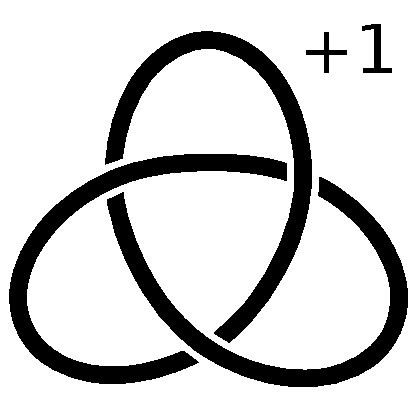
\includegraphics[width=0.5\linewidth]{./pictures/right_handed_trefoil_+1_surgery.pdf}
		\end{center}
		\caption{
			A Kirby diagram for $X_{n}(K)$ is given just by the knot $K$ with the framing $n$ written next to it.
			For example, here is a Kirby diagram representing the $1$-trace
			$X_1(\textrm{right handed trefoil})$.
			The boundary of this $4$-manifold is the $+1$-surgery
			$\sphere{3}_{+1}(\textrm{right handed trefoil})$,
			a possible description of the Poincar\'e homology sphere.}
		\label{fig:right_handed_trefoil_+1_surgery}
	\end{marginfigure}
\end{definition}

\begin{theorem}[{\citep[Thm. 1.8]{miller2018knot}}]
	\begin{itemize}
		\item $K$ is smoothly slice if and only if $X_{0}(K)$ smoothly embeds in $\sphere{4}$.
		\item Similarly, $K$ is topologically slice if and only if $X_{0}(K)$ topologically
		embeds in $\sphere{4}$.
	\end{itemize}
\end{theorem}

\begin{remark}[Exotic $\RR^{4}$ from a topologically, but
	not smoothly slice knot]
	References:
	\citep{57926}
	%TODO
	TODO
	
	Observe that this construction gives a \textit{large}
	\index{exotic $\RR^{4}$!large}
	exotic $\RR^{4}$ since it contains the compact subset
	$X_{0}(K)$ which does not embed smoothly in
	$\RR^{4}_{\mathrm{std}}$.
\end{remark}


\begin{definition}
	A knot $K$ is called \textit{doubly slice} \index{knot!doubly slice}
	if it occurs as an
	equatorial\sidenote{
		$\sphere{3} \subset \sphere{4}$ is the standard inclusion
		of the equator.
	} cross section
	\[
		K = S \cap \sphere{3}
	\]
	of an unknotted topologically locally flat
	$2$-sphere $S^{2} \subset \sphere{4}$
	embedded in the $4$-sphere.\marginnote{
			A double slice knot slices in two
			different ways.
		}
\end{definition}

\begin{lemma}[\citep{friedl2quick}, \citep{friedl2015twist}]
	$K \# -K$ is smoothly doubly slice.
\end{lemma}

\begin{remark}
	We can use the standard spinning of this knot to obtain a $2$-sphere
	with cross-section $K \# -K$, but this $\sphere{2} \subset \sphere{4}$
	will be knotted in general.
	We can see this because its knot group 
	is the same as the one of the knot we started with.
	So we cannot use this ``obvious'' sphere to prove that $ K \# -K $ knot is doubly slice.
	
	As an alternative, we can use the (more complicated)
	$\pm 1$-twist spin of our knot to obtain an unknotted
	sphere in $\sphere{4}$ with cross-section
	$K \# -K$ \citep{zeeman1965twisting}.
	
\end{remark}


\begin{definition}
	A knot $K \subset \sphere{3}$ is \textit{homotopy ribbon} \index{knot!homotopy ribbon}
	if there is a slicing disk $\Delta^{2} \subset \disk{4}$
	for with the inclusion of the knot exterior into
	the slice disc exterior induces a surjection on fundamental groups,
	\begin{equation*}
		\pi_1( \sphere{3} \setminus K )
		\twoheadrightarrow
		\pi_1( \disk{4} \setminus \Delta )
	\end{equation*}
\end{definition}


\subsection{Concordance of Links}

\begin{definition}
	A \textit{smooth link cobordism} \index{link!cobordism} between the links
	$L_0, L_1 \subset \sphere{3}$
	is a smooth, compact, oriented surface
	$\Sigma$ generically embedded in $\sphere{3} \times \interval$ such that
	$\partial \Sigma = \overline{L_{0}} \coprod L_{1}$,
	where $\partial \Sigma \subset \sphere{3} \times \{0, 1\}$.
\end{definition}

\begin{proposition}
	Linking numbers are concordance invariants.
\end{proposition}

\begin{remark}[The Hopf link is ``the most non-slice link'', \citep{krushkal2015slicing}]
	Any link in $\sphere{3}$ bounds immersed smooth disks
	$\coprod^{n} \disk{2} \looparrowright \disk{4}$.
	%TODO
	TODO
\end{remark}


\begin{definition}[Boundary link]
	\marginnote{It is possible that each component
		of a link bounds a Seifert surface missing the other components,
		but still they do not bound disjoint surfaces.}
	A link $L^{n} \subset \sphere{n+2}$ whose components bound disjoint Seifert surfaces
	is called a \textit{boundary link} \index{link!boundary}.
\end{definition}

\begin{example}
	The untwisted Bing double of any knot is a boundary link.
	%TODO
	TODO Insert definition of Bing double
	TODO Insert picture
	TODO Proof that Bing doubles are boundary links
	(draw the taco shells, need 4 copies of the Seifert surface
	of the knot)
\end{example}

\begin{proposition}[{\citep[5.E.1]{rolfsen2003knots}}]
	If any two components of $L^{1} \subset \sphere{3}$
	have nonzero linking number, then $L$ is \textbf{not}
	a boundary link.
\end{proposition}

\begin{proof}
	Use the definition \ref{def:linking_numbers_via_intersections_with_Seifert_surface} 
	of linking number where you count
	the intersection points of one component with a Seifert surface for the
	other.
\end{proof}

\begin{definition}[{Linking number via intersections with a Seifert surface,
	\citep[5.D.(2)]{rolfsen2003knots}}]
	\label{def:linking_numbers_via_intersections_with_Seifert_surface}
	Let $J$ and $K$ be two disjoint oriented knots (e.g. link components).
	Pick a PL Seifert surface $M^{2}$ for $K$, with
	a bicollar $(N, N^{+}, N^{-})$ of the interior $\mathring{M}$.
	Make $J$ transverse to $M$, i.e. assume after a small
	homotopy of $J$ in $\sphere{3} \setminus K$ that
	$J$ meets $M$ in a finite number of points
	and that at each point $J$ passes locally
	from $N^{+}$ to $N^{-}$ or from $N^{-}$ to $N^{+}$.
	Corresponding to this direction, weight the intersection types
	with $+1$ or $-1$.
	\marginnote{On first sight this seems to depend on the
	choice of Seifert surface $M$.}
	The signed sum of these intersection points is the linking
	number $\lk(J, K) \in \Z$.
\end{definition}

\begin{proposition}[{\citep[5.E.8]{rolfsen2003knots}}]
	If a link $L$ is a boundary link, then each component
	represents an element
	in the second commutator subgroup\sidenote{Also called
		\textit{second derived subgroup} or $G^{(2)}$,
		it is generated by elements of
		the form $[[x,y],[z,w]]$.}
	of the fundamental group of the complement
	of the remaining component(s).
\end{proposition}

\subsection{The Cappell-Shaneson way to slice a knot}

\citep[4.1]{Teichner2010}

\begin{definition}
	A knot $K \colon \sphere{1} \subset \sphere{3}$ which is slice in a homology $4$-ball
	is called \textit{homologically slice}.
	\marginnote{
		\begin{openquestion*}[\textcolor{olive}{(Still open?)}]
			Find an obstruction which is able to tell the
			difference between homologically slice and actually slice.
		\end{openquestion*} }
\end{definition}


\subsection{Heegaard Floer homology}

The concordance invariant $\tau(K) \in \Z$ for a knot $K \subset \sphere{3}$
is defined in \citep{ozsvath2003knot},
this yields a homomorphism $\mathcal{C} \rightarrow \Z$.

%TODO
TODO Explain this definition
\begin{definition}[Ozsv\'ath and Szab\'o's $\tau$-invariant]
	\begin{equation*}
		\tau(K) = \min \{ i \in \Z \mid 
			H_{*}(\mathcal{F}(K, i))
			\rightarrow
			\widehat{HF}(\sphere{3}) 
			\textrm{ is nontrivial} \}
	\end{equation*}
\end{definition}

Properties of $\tau$:
\begin{itemize}
	\item It provides a lower bound for the four-ball genus,
	\[
		| \tau(K) | \le g_{4}(K)
	\]
	\item TODO %TODO
\end{itemize}


\begin{definition}[\citep{hom2011note}]
	An \textit{L-space} \index{L-space} is a rational homology 3-sphere\sidenote{$Y^{3}$ is a rational homology sphere
		iff $H_{1}(Y; \mathbb{Q}) = 0$, which means that the first homology with integer coefficients
		is a finite group.}
	with the simplest possible Heegaard-Floer homology,
	\begin{equation*}
		\dim \widehat{HF}(Y) = | H_{1}(Y ; \Z) |.
	\end{equation*}
	\marginnote{For any rational homology $3$-sphere
		$\rk \widehat{HF}(Y) \ge | H_{1}(Y ; \Z) |$,
		and L-spaces are those for which this bound is sharp.}
	
	A knot admitting a non-trivial L-space surgery is
	called an \textit{L-space knot}
	\index{knot!L-space}.
\end{definition}

\begin{example}
	\begin{itemize}
		\item Lens spaces are L-spaces (and this is also where the
		name comes from).
		
		\item Torus knots are L-space knots, as
		$pq \pm 1$ surgery on the $(p,q)$-torus knot yields a
		lens space. 
		%TODO
		\marginnote{TODO Why?}
	\end{itemize}
\end{example}

\newpage

\subsection{The Algebraic Concordance Group}

\begin{definition}
	Let $A, B$ be square integral matrices.
	$A$ is called \textit{cobordant} \index{matrix!cobordant} to $B$
	if $A \oplus (-B)$ is hyperbolic.\marginnote{
		$A$ congruent to $B$ implies $A$ cobordant to $B$.}
\end{definition}

\begin{remark}
	\begin{itemize}
		\item Cobordism of matrices is reflexive and symmetric
		\item For transitivity one has to impose the extra restriction that
		$\det(A - A^{T}) \ne 0$ (but this is always satisfied for Seifert matrices
		$A$ because $A - A^{T}$ represents the intersection form on a basis for the
		first homology) and the following lemma
	\end{itemize}
\end{remark}

\begin{lemma}[Stable hyperbolic implies hyperbolic / Cancellation]
	Suppose $A, N$ are square and $det(N - N^{T}) \ne 0$.
	If $A \oplus N$ and $N$ are hyperbolic, then $A$ is hyperbolic.
\end{lemma}

%TODO Continue with facts about the algebraic cobordism group


\newpage
% ----------------------
\section{Property P and R}
% ----------------------

\begin{definition}[Property P, \citep{kirby1978slice}]
	If (nontrivial) Dehn surgery on a knot
	cannot yield a homotopy $3$-sphere
	then the knot is said to satisfy
	\textit{Property P} \index{Property!P}.
\end{definition}

\begin{theorem}[Kronheimer, Mrowka]
	All knots, except the unknot, have Property P.
\end{theorem}

\begin{definition}[Property R]
	If $0$-framed surgery on a knot cannot yield
	$\sphere{1} \times \sphere{2}$ then it
	satisfies
	\textit{Property R} \index{Property!R}.\marginnote{
			We could also drop the condition
			that the framing is assumed to be
			trivial: It is clear from looking at the
			intersection pairing on the trace of the surgery
			that if the result is $\sphere{1} \times \sphere{2}$,
			the framing had to be $0$.
			%TODO More details?
		}
\end{definition}

\begin{theorem}[Gabai]
	If $0$-framed surgery on $K \subset \sphere{3}$ is 
	$\sphere{1} \times \sphere{2}$
	then $K$ is the unknot\sidenote{
			In other words:
			All knots, except the unknot, have Property R.
		}.
\end{theorem}


\begin{conjecture}[Generalized Property R, \citep{scharlemann2009fibered},
	{\citep[Problem 1.82]{kirby1995problems}}]
	Suppose $L \subset \sphere{3}$ is an $n$-component
	link with integer framings, and surgery on $L$ gives
	the connected sum $ \#^{n} (\sphere{1} \times \sphere{2}) $.
	
	Then there is a sequence of handle slides on $L$
	that converts $L$ into a $0$-framed unlink.
\end{conjecture}

\begin{remark}
	\begin{itemize}
		\item For $n$=1, i.e. a single component, there are no slides
		possible and the statement is Gabai's theorem.
		
		\item For $n > 1$ it is necessary to include the possibility
		of handle slides into the theorem.
		For an example, you can use Kirby moves
		on a zero framed unlink to complicate the link.
		
		\item The only framed links that are relevant for the
		conjecture are those where all framings and linking
		numbers are trivial.
	\end{itemize}
\end{remark}





\newpage
% ----------------------
\section{Satellite operators}
% ----------------------

\citep{cochran2014injectivity}

Let $P$ be an oriented knot in the solid torus $\sphere{1} \times \disk{2}$,
this is called a \textit{pattern knot} \index{knot!pattern}.
For $K$ an oriented knot in $\sphere{3}$ we denote by $P(K)$
the (untwisted) \textit{satellite} \index{knot!satellite} of $K$
with pattern $P$. The knot $K$ is sometimes called
a companion\sidenote{You can imagine that the satellite knot
	is orbiting its companion.}
of $P(K)$ \citep[p. 10]{lickorish2012introduction}.

An important special case of satellites are
\begin{definition}[$(p,q)$-cables]
	The \textit{$(p,q)$-cable} of a knot $K$
	\index{knot!cable},
	denoted by $K_{p, q}$
	is the satellite knot with pattern the $(p, q)$-torus knot.
	$p$ is the number of times $K_{p, q}$ transverses
	the longitudinal direction of $K$,
	and $q$ the meridional number.
\end{definition}

We can view a pattern as a function
\begin{equation*}
	P \colon \mathcal{K} \rightarrow \mathcal{K}
\end{equation*}
\marginnote{$\mathcal{K} =
	\frac{ \{ \textrm{knots } \sphere{1} \hookrightarrow \sphere{3} \} }{\textrm{isotopy}}$}
on the set of isotopy classes of
knots.
These descent to yield functions (\textit{satellite operators})
\begin{equation*}
	\mathcal{K} / \sim \rightarrow \mathcal{K}/ \sim
\end{equation*}
for various equivalence relations $\sim$ on $\mathcal{K}$, for example
concordance.

%TODO
If $K$ and $J$ are concordant, their satellites will be concordant
via a concordance which ``follows along'' the concordance between
$K$ and $J$.
%TODO



% ----------------------
\section{Braid groups}
% ----------------------

\begin{exercise}
	Show that there is a presentation for the braid groups
	with just two generators.
\end{exercise}

\begin{definition}[\citep{hedden2010notions}]
	A knot which has a diagram with only positive crossings
	is called a \textit{positive knot} \index{knot!positive}.
	\marginnote{Equivalently, a knot is positive
		if it has a projection for which the writhe
		is equal to the crossing number.}
	
	\textit{Positive braids} \index{braid!positive} are those
	knots and links which can be obtained as the closure
	of a word in the braid group containing
	only positive generators\sidenote{I.e.\ closures of
		products $ \prod\limits_{k=1}^{m} \sigma_{i_{k}} $,
		where there are no $\sigma_{i}^{-1}$,
		and $\sigma_{i}$ is a positive Artin generator.}.
	
	A \textit{quasi-positive braid} \index{braid!quasi-positive}
	is a braid that is a product of 
	conjugates of positive generators\sidenote{
		I.e.\ as products of positive bands
		$\alpha \cdot \sigma_{j} \cdot \alpha^{-1}$,
		where $\alpha \in B_{n}$ is an arbitrary braid word}.
	
	A knot is called
	\textit{quasi-positive} \index{knot!quasi-positive}
	if it is the
	closure of a quasi-positive braid.
	\marginnote{Quasipositive knots are closures
		of braids consisting of arbitrary conjugates of positive generators.
		
		Strongly quasipositive knots require these conjugates
		to be of a special form useful for constructing
		Seifert surfaces.}
\end{definition}



% ---------------------------------------------------
\section{TQFTs - Topological Quantum Field Theories}
% ---------------------------------------------------


%TODO
TODO Write down axioms

\marginnote{A monoidal functor is supposed to preserve the identity
objects for the tensor product. Since the empty set is the identity for the tensor product in the bordism category (given by disjoint union of the bordisms), the TQFT should send this to the identity object for
$\otimes_{R}$, which is just the ground ring $R$.}



\newpage
% ----------------------
\section{$2$-Knots}
% ----------------------
\begin{definition}[$n$-concordance]
	A $2$-knot $K$ is
	\emph{$n$-concordant} \index{$n$-concordance}
	to $K'$
	if there is a properly embedded ``annulus''
	$\sphere{2} \times [0,1] \hookrightarrow \sphere{4} \times [0,1]$
	which restricts to the $2$-knots
	$K = \sphere{2} \times [0, 1] \cap \sphere{4} \times \{ 0 \}$
	and
	$K' = \sphere{2} \times [0, 1] \cap \sphere{4} \times \{ 1 \}$
	on both ends,
	and such that every level set consists
	of surfaces of maximum genus $n$.
\end{definition}
\begin{definition}[$n$-cobordism]
	Same as $n$-concordance, only we
	\underline{don't} assume that the properly embedded
	$3$-manifold interpolating
	between the two boundary sides is an annulus.
\end{definition}
\begin{remark}[Warning]
	Sometimes the words
	\emph{cobordism} and \emph{concordance}
	are used interchangeably,
	but here they mean very different things
	(``annulus'' $\sphere{2} \times [0, 1]$ versus
	arbitrary $3$-manifold $M^{3}$).
\end{remark}



\newpage
% ----------------------
\section{Open questions}
% ----------------------

\begin{openquestion}
	Is the crossing number of a satellite knot bigger than that of its companion?
\end{openquestion}

\begin{openquestion}[Smooth unknotting conjecture]
	A $2$-knot is trivial if and only if the fundamental group
	is infinite cyclic.
\end{openquestion}

\begin{remark}
	\begin{itemize}
		\item It is proved that a $2$-knot exterior
		is homotopy equivalent to $\sphere{1}$ if and only if
		the fundamental group is infinite cyclic
		
		\item Freedman proved the unknotting conjecture in the
		topological category,
		but it is still open in the piecewise-linear or smooth
		category
	\end{itemize}
\end{remark}



\subsection{Open Questions in Knot concordance}

A list of knots whose sliceness status is (supposedly) not known:
\begin{enumerate}
	\item $(2, 1)$-cable on the figure eight
	\item Negative Whitehead double of the right handed trefoil
	\item Positive Whitehead double of the left handed trefoil
	\item Any Whitehead double of the figure eight
	\item ...
\end{enumerate}


\subsection{Current developments/Recently solved}

\begin{itemize}
	\item The Conway knot $11n34$ is not slice, as shown
	in \citep{piccirillo2018conway}
	
	\item Kronheimer and Mrowka found an error
	in their paper \citep{kronheimer2013gauge} which
	(incorrectly?) claimed that Rasmussen's $s$-invariant could
	not detect an exotic $4$-ball. \\
	In particular the methods of
	\citep{freedman2009man} could possibly lead
	to an
	exotic $4$-sphere.
	
\end{itemize}
% % % % % % % % % % % % % % % % % % % % % % % % %

% % % % % % % % % % % % % % % % % % % % % % % % %
% % % % % % % % % % % % % % % % % % % % % % % % %
\chapter{4-Manifolds}
% % % % % % % % % % % % % % % % % % % % % % % % %

% ----------------------
\section{Bordism}
% ----------------------

\begin{definition}
	The $n$-dimensional oriented \textit{cobordism group}
	\index{cobordism group}
	over the space $X$ is
	\begin{equation*}
		\Omega_{n}[X] =
			\frac{ \{ f \colon M^{n} \rightarrow X \mid M^n \textrm{ oriented, closed, } 
			n\textrm{-dim. manifold} \}}{\textrm{bordism}}
	\end{equation*}
	\marginnote{If $\alpha \colon M^{n} \rightarrow X$
		represents a bordism class, $M^n$ is allowed to
		have more than one component.}
\end{definition}

\begin{proposition}[{\citep[13.15, p. 319]{kauffman1987knots}}]
	\begin{itemize}
		\item Pushing forward a fundamental class
		\begin{align*}
			\Omega_n [X] & \rightarrow H_{n}(X ; \Z) \\ 
			[f \colon M^{n} \rightarrow X] & \mapsto f_{*}([M])
		\end{align*}
		is an isomorphism for $n \le 3$.
		
		\item The sequence
		\begin{equation*}
			\Omega_{4}[\ast] \rightarrow \Omega_{4}[X] \rightarrow H_{4}(X ; \Z)
		\end{equation*}
		is exact.
	\end{itemize}
\end{proposition}

%TODO

% ------------------------------------
\section{Mazur manifolds}
% ------------------------------------

\textbf{References}:
\begin{itemize}
	\item Homology spheres: \citep{saveliev2013invariants}
	\item \citep{akbulut1979mazur}
\end{itemize}

%TODO
TODO


% ------------------------------------
\section{Andrews-Curtis Conjecture}
% ------------------------------------

\citep{SCP4}

\begin{definition}
	A \textit{balanced presentation} \index{presentation!balanced} is a presentation
	\[
		\langle g_1, \ldots, g_n \mid r_1, \ldots, r_n \rangle
	\]
	with the same number of generators and relations.
	
	The Andrew-Curtis moves on a balanced presentation are
	\begin{enumerate}[label=(\roman*)]
		\item \textbf{1-handle slides:} Replace a pair of generators
		$ \{ x, y \} $ by $ \{ x, xy \} $
		
		\item \textbf{2-handle slides:} Replace a pair of relations
		$ \{ r, s \} $ by $ \{ grg^{-1}s, s \} $, where $ g $ is any word in the generators
		
		\item \textbf{1-2-handle cancellations:} Add a generator together with
		a new relation killing it
	\end{enumerate}
	In particular, you are \underline{not} allowed to make a copy of a relation to
	keep for later use (which would correspond to 
	\textbf{2-3-handle creation/cancellation}).
\end{definition}

\begin{conjecture*}[Andrews-Curtis conjecture \textcolor{red}{(Probably false?)}]
	Any balanced presentation of the trivial group can be transformed
	by Andrews-Curtis moves to the trivial presentation.
\end{conjecture*}

\begin{example}
	%TODO
	TODO
	\[
		\langle x, y \mid xyx = yxy, x^{5} = y^{4} \rangle
	\]
	is a balanced presentation of the trivial group,
	but until now nobody was able to find a sequence of
	Andrews-Curtis moves to transform it into the trivial presentation
	\[
		\langle x, y \mid x, y \rangle
	\]
\end{example}

%TODO
TODO
Explain how to construct homotopy $4$-spheres from balanced
presentations of the trivial group
\citep{akbulut1985potential}

\marginnote{
	In \citep[I.3]{kirby2006topology} Kirby suspected that the
	\textit{Dolgachev surface}
	\index{Dolgachev surface} $E(1)_{2,3}$ 
	(an exotic copy of the rational elliptic surface
	$ \CP{2} \# 9 \overline{\CP{2}} $)
	might require 1- and/or 3-handles.
	But in \citep{akbulut2008dolgachev} Akbulut found a
	handlebody presentation without those.
}
\begin{openquestion*}[]
	Does a simply connected, closed, smooth $4$-manifold need
	$1$-handles and/or $3$-handles?
\end{openquestion*}

\begin{observation}
	If exotic $\sphere{4}$ exist, their handle decomposition must
	contain $1$- or $3$-handles.
	
	For this suppose you have a handle decomposition of a manifold
	with the homology of $\sphere{4}$ and no $1$- and $3$-handles,
	then there could not be any $2$-handles either because these would
	give nontrivial second homology. 
\end{observation}

\begin{definition}
	Use the following notation to denote the abelian group
	\begin{equation*}
		\Gamma_n = 
		\frac{\textrm{orientation preserving diffeomorphisms of } \sphere{n-1}}
			 {\textrm{those that extend to a diffeomorphism of } \disk{n}}
	\end{equation*}
\end{definition}
\marginnote{
	\begin{itemize}
		\item $\Gamma_{1} = \Gamma_{2} = 0$
		\item Munkres, Smale: $\Gamma_{3} = 0$
		\item Cerf: $\Gamma_{4} = 0$
		\item Kervaire, Milnor: $\Gamma_{5} = \Gamma_{6} = 0$,
		$\Gamma_{7} = \Z / 28$
	\end{itemize}
	}

\begin{proposition}
	For $n \ge 5$ we can identify $\Gamma_{n}$
	with the set of oriented smooth structures
	of the topological $n$-sphere.
	I.e. in dimension $\ge 5$ all exotic spheres
	can be obtained by using a diffeomorphism of
	$\sphere{n-1}$ to glue two $n$-disks along their boundary.
\end{proposition}

\begin{theorem}[Cerf, \citep{geiges2010eliashberg}]
	Any diffeomorphism of the $3$-sphere $\sphere{3}$
	extends over the $4$-ball $\disk{4}$,
	in other words
	\[
		\Gamma_4 = 0.
	\]
\end{theorem}

\begin{observation}
	Cerf's theorem implies that there are no exotic structures
	on $\sphere{4}$ that can be obtained by gluing
	two $4$-disks along their
	boundary.
\end{observation}





\newpage
% ------------------------------------
\section{Trisections}
% ------------------------------------

\begin{center}
	\textsc{``Trisections are to $4$-manifolds as Heegaard splittings are to
		$3$-manifolds''}
\end{center}

\subsection{References}

\begin{itemize}
	\item Original paper: \citep{gay2016trisecting}
	\item Lecture notes: \citep{gay2019heegaard}
\end{itemize}

\subsection{Definitions}

\marginnote{
	\begin{itemize}
		\item $\#^n A$ is the connected sum of $n$ copies of $A$,
		with $\#^{0} A = \sphere{m}$
		
		\item TODO
		%TODO
	\end{itemize}}
\begin{definition}
	\begin{itemize}
		\item The standard genus $g$ surface is
		\[
			\Sigma_g = {\#}^{g} (\sphere{1} \times \sphere{1})
		\]
		\item The standard genus $g$ solid handlebody is
		\[
			H_g = \natural^g (\sphere{1} \times \disk{2})
		\]
		with $\partial H_{g} = \Sigma_{g}$
		\marginnote{$\partial (A \natural B) = (\partial A) \# (\partial B)$}
		
		\item The standard $4$-dimensional $1$-handlebody
		(of ``genus $k$'') is
		\[
			Z_{k} =\natural^{k} (\sphere{1} \times \disk{3})
		\]
		i.e.\ a $4$-ball to which we attach $k$-many
		$4$-dimensional $1$-handles.
	\end{itemize}
\end{definition}
\begin{marginfigure}
	\begin{center}
		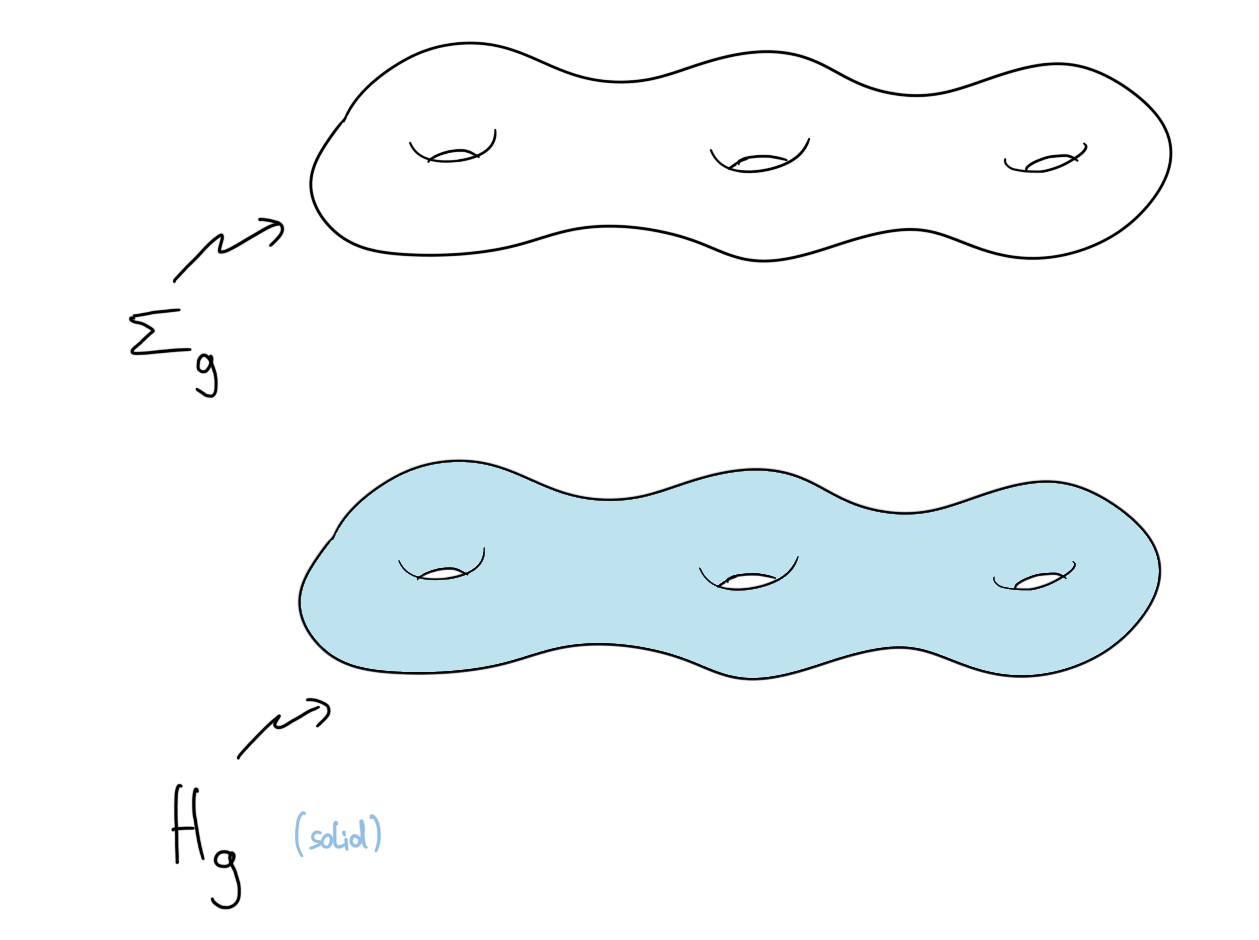
\includegraphics{./pictures/standard_manifolds.png}
	\end{center}
	\caption{Standard manifolds of dimension 2, 3}
	\label{fig:standard_manifolds}
\end{marginfigure}
% % % % % % % % % % % % % % % % % % % % % % % % %

% % % % % % % % % % % % % % % % % % % % % % % % %
\chapter{Topics to study and Reading List}

\section{Questions}

%TODO
\begin{itemize}
	\item TODO
\end{itemize}


\section{Reading List}

\begin{itemize}
	\item List of open problems concerning quantum invariants
		is at
		\citep{ohtsuki2002problems}
		
	\item Vassiliev knot invariants, for this
		\citep{bar1995vassiliev}
		
	\item Khovanov homology
		\citep{bar2005khovanov}
	
	\item Kaufman's books, for example
		\citep{kauffman2001knots}
		
	\item Baez's book on gauge theory
		\citep{baez1994gauge}
\end{itemize}
% % % % % % % % % % % % % % % % % % % % % % % % %


%----------------------------------------------------------------------------------------

\backmatter

%----------------------------------------------------------------------------------------
%	BIBLIOGRAPHY
%----------------------------------------------------------------------------------------

\bibliography{mybib} % Use the mybib.bib file for the bibliography

%----------------------------------------------------------------------------------------

\printindex % Print the index at the very end of the document

\end{document}
